\documentclass[9pt,a4paper,twocolumn,twoside]{tau-class/tau}
\usepackage[english]{babel}
\usepackage{tikz}

%----------------------------------------------------------
\doctype{ABB Industrial Hackathon 2026 — Submission}
\title{DRIVEWISE — Multi-Drive Industrial Simulation \& Validation Platform}

\author[a,1]{Aashaya Gautam\thanks{\href{mailto:gautam_aashaya@srmap.edu.in}{gautam\_aashaya@srmap.edu.in}\enspace|\enspace\href{https://github.com/GrimDocDimes/DRIVEWISE}{github.com/GrimDocDimes/DRIVEWISE}}}


\docinfo{DRIVEWISE is a digital-twin simulation of ABB ACS880 coordinated conveyor drives featuring predictive maintenance analytics, automated Factory Acceptance Testing, and an ISA-101 compliant high-performance HMI — built with React~18, Python~3.12, WebSocket, and Apache ECharts.}

\footinfo{DRIVEWISE v1.0}
\organization{SRM University -- AP}
\leadauthor{Aashaya Gautam}

%----------------------------------------------------------

\begin{abstract}
    DRIVEWISE is a high-fidelity multi-drive industrial simulation platform that models three coordinated ABB ACS880 variable frequency drives controlling a bulk material conveyor system. Unlike conventional single-motor demonstrations, DRIVEWISE simulates ABB's patented Direct Torque Control algorithm, dual-node motor thermal dynamics with Arrhenius insulation degradation, conveyor belt physics with slip detection, and bearing vibration diagnostics with ISO~10816 severity classification. The platform delivers a 7-screen ISA-101 compliant operator interface, an automated 6-test Factory Acceptance Test engine with PDF report generation, and predictive maintenance analytics that directly mirror ABB Ability Smart Sensor functionality — constituting a complete virtual commissioning environment for industrial drive system validation.
\end{abstract}

\keywords{ABB ACS880, Direct Torque Control, multi-drive coordination, predictive maintenance, ISA-101 HMI, Factory Acceptance Testing, digital twin, virtual commissioning}

%----------------------------------------------------------

\begin{document}

\maketitle
\thispagestyle{firststyle}

%===========================================================
% PAGE 1 — INPUTS CONSIDERED
%===========================================================

\section{Inputs Considered}

\taustart{D}RIVEWISE was designed by studying the actual engineering workflows ABB uses to commission coordinated drive systems in mining, ports, and bulk material handling. Every input maps directly to an ABB product, an industrial standard, or verified physics. The platform simulates what ABB actually sells and deploys — not what textbooks describe.

\subsection{Industrial Domain Inputs}

\begin{itemize}
    \item \textbf{ABB ACS880 drive architecture} — Direct Torque Control (DTC), the patented core technology inside every ACS880 unit, achieving $\pm$0.1\% speed accuracy with sub-millisecond torque response
    \item \textbf{Multi-drive conveyor topology} — 3-section bulk material conveyor system (Infeed $\rightarrow$ Transfer $\rightarrow$ Discharge) with master-follower speed coordination — one of ABB's largest drive deployment verticals
    \item \textbf{Motor nameplate data} — 75\,kW, 415\,V, 135\,A, 1475\,RPM, 4-pole squirrel-cage induction motor rated per IEC~60034
    \item \textbf{Conveyor mechanical profile} — 5000\,kg belt mass, 8000\,kg maximum material load, 0.6\,m drive pulley, 15:1 helical gear reduction
    \item \textbf{6203-2Z bearing specification} — Ball pass frequencies (BPFO/BPFI/BSF) for defect detection, ISO~10816 vibration severity classification scale
\end{itemize}

\subsection{Physics Model Inputs}

\begin{itemize}
    \item \textbf{Drive model} — DTC torque/flux control loop at 25\,$\mu$s equivalent cycle time, S-curve ramp generator with configurable jerk limiting, scalar V/f fallback mode for basic applications
    \item \textbf{Motor thermal model} — Dual-node stator/rotor thermal equivalent circuit, $I^2R$ copper winding losses, core losses from eddy currents and hysteresis, speed-dependent forced cooling coefficient
    \item \textbf{Conveyor dynamics} — Newton's rotational second law: $J\frac{d\omega}{dt} = T_{\text{motor}} - T_{\text{load}}$, belt slip detection via motor-to-belt speed differential exceeding 5\%
    \item \textbf{Bearing vibration} — Synthetic FFT spectrum with characteristic defect frequency injection at amplitudes growing over simulated operating hours following a Weibull degradation curve
    \item \textbf{Variable load profile} — 12-point cyclic material load pattern simulating crusher-feed variations, live-configurable from HMI during runtime
\end{itemize}

\subsection{Standards \& Design Inputs}

\begin{itemize}
    \item \textbf{IEC 60255} — Inverse-time overcurrent protection characteristics (curve B), governing trip time as a function of overcurrent magnitude
    \item \textbf{IEC 61131-3} — PLC start/stop sequencing with permissive logic, multi-drive fault cascade response rules
    \item \textbf{ISA-18.2} — Alarm management lifecycle states: Inactive $\rightarrow$ Active/Unacknowledged $\rightarrow$ Acknowledged $\rightarrow$ Return to Normal
    \item \textbf{ISA-101} — High-performance HMI design principles: colour communicates \textit{abnormality}, not identity; grey-state normal operation
    \item \textbf{Arrhenius equation} — Thermal insulation life degradation model: $\text{Life} = A \cdot e^{E_a / (k_B T)}$, the industrial standard for motor insulation aging
\end{itemize}

\subsection{Technology Stack}

\begin{itemize}
    \item \textbf{Frontend:} React 18 + Vite 5 + Apache ECharts (canvas-rendered, industrial-grade charting library)
    \item \textbf{Backend:} Python 3.12 async simulation engine with NumPy for numerical computation
    \item \textbf{Communication:} WebSocket protocol at 100\,ms broadcast interval (10\,Hz real-time tag streaming)
    \item \textbf{Reports:} ReportLab PDF generation for formal Factory Acceptance Test documentation
    \item \textbf{Design:} ISA-101 dark palette (\texttt{\#1A1A3E} background), monospace typography, Lucide icon system
\end{itemize}

\begin{tauenv}[frametitle=Key Innovation — What Separates DRIVEWISE From Every Other Submission]
Most teams simulate one motor turning on and off with a speed number on screen. \textbf{DRIVEWISE simulates what ABB actually sells and deploys} — a coordinated multi-drive system where three ACS880 drives work together on a shared mechanical load, with energy optimisation running continuously, predictive maintenance tracking motor health in real time, and the entire system validated automatically against a 6-test Factory Acceptance Test suite \textit{before a single piece of hardware is touched}. The platform is a \textbf{virtual FAT environment} — the same concept ABB uses internally to validate drive systems before shipping to site.
\end{tauenv}

%===========================================================
% PAGES 2–4 — PROCESS FOLLOWED
%===========================================================

\section{Process Followed}

\subsection{System Architecture Design}

The platform follows a three-tier industrial architecture that directly mirrors real-world SCADA deployment patterns used in ABB 800xA and similar distributed control systems:

\begin{figure}[H]
\centering
\small
\begin{tikzpicture}[
  box/.style={draw=taucolor,fill=taucolor!5,rounded corners=2pt,minimum height=7mm,
              font=\scriptsize\sffamily\bfseries,text=taucolor,align=center},
  arr/.style={->,thick,taucolor}
]
  \node[box,minimum width=82mm,fill=blue!4] (hmi) at (0,2) {Level 3: React HMI — 7 ISA-101 Screens};
  \node[box,minimum width=55mm,fill=green!4] (ws) at (0,1) {WebSocket Bridge — 100\,ms (ws://8765)};
  \node[box,minimum width=18mm] (drive) at (-2.8,0) {Drive\\(DTC)};
  \node[box,minimum width=18mm] (motor) at (-0.9,0) {Motor\\(Thermal)};
  \node[box,minimum width=18mm] (conv) at (0.9,0) {Conveyor\\(Inertia)};
  \node[box,minimum width=18mm] (bear) at (2.8,0) {Bearing\\(FFT)};
  \node[box,minimum width=82mm,draw=red!60,fill=red!3] (coord) at (0,-0.9) {Coordinator: 3 Units $\times$ 4 Models + 5 Protections};
  \draw[arr] (hmi.south) -- (ws.north);
  \draw[arr] (ws.south) -- ++(0,-0.2) -| (drive.north);
  \draw[arr] (ws.south) -- ++(0,-0.2) -| (motor.north);
  \draw[arr] (ws.south) -- ++(0,-0.2) -| (conv.north);
  \draw[arr] (ws.south) -- ++(0,-0.2) -| (bear.north);
  \draw[arr] (drive.south) -- ++(0,-0.15) -| (coord.north -| drive);
  \draw[arr] (motor.south) -- ++(0,-0.15) -| (coord.north -| motor);
  \draw[arr] (conv.south) -- ++(0,-0.15) -| (coord.north -| conv);
  \draw[arr] (bear.south) -- ++(0,-0.15) -| (coord.north -| bear);
\end{tikzpicture}
\caption{Three-tier architecture: Physics $\rightarrow$ WebSocket $\rightarrow$ HMI.}
\label{fig:arch}
\end{figure}

\textbf{Level 1 (Physics Engine):} Python 3.12 async simulation running 12 model instances (3 units $\times$ 4 models each) with coordinated master-follower logic and 5 protection functions. Each 10\,ms simulation step advances all physics simultaneously.

\textbf{Level 2 (Communication):} WebSocket bridge on port 8765 broadcasts a JSON tag snapshot every 100\,ms to all connected HMI clients. A bidirectional command channel handles start/stop, parameter changes, fault injection, configuration updates, and test execution commands.

\textbf{Level 3 (HMI):} React 18 single-page application with 7 ISA-101 compliant screens, Apache ECharts for industrial trending, and real-time WebSocket subscription for live data display.

\subsection{Physics Simulation Engine (Python)}

\subsubsection{Drive Model — ABB DTC Emulation}

The ACS880 drive model implements two control modes. In \textbf{DTC mode}, the drive directly controls motor torque and magnetic flux, achieving $\pm$0.1\% speed accuracy with sub-millisecond torque step response — fundamentally different from standard V/f drives which control voltage and frequency indirectly. In \textbf{Scalar V/f mode}, a fixed voltage-to-frequency ratio is maintained for basic pump/fan applications where precise speed control is not critical.

The \textbf{S-curve ramp generator} implements configurable acceleration time, deceleration time, and emergency stop ramp — not simple linear ramps, but S-curve profiles with jerk limiting to prevent mechanical shock on belt joints and gearboxes. An operator can tune all parameters from the HMI and observe the effect on speed response in real time.

\subsubsection{Motor Thermal Model}

A dual-node thermal equivalent circuit models stator winding temperature ($I^2R$ copper losses) and rotor temperature (core losses from eddy currents and hysteresis) with independent thermal masses and heat transfer cross-coupling through the air gap.

Cooling is speed-dependent: at rated speed, forced convection from the shaft-mounted fan provides maximum cooling. At zero speed, only natural convection operates — a critical distinction because motors running at low speed under load overheat much faster. The thermal model produces realistic trip timing that matches IEC~60255 inverse-time curves.

\textbf{Arrhenius insulation degradation} tracks cumulative thermal stress over all operating cycles: every hour the motor runs above its rated temperature class, insulation life is consumed at an exponentially accelerating rate. The dashboard displays remaining insulation health as a declining percentage — the same metric ABB Ability Smart Sensor reports on real motors.

\subsubsection{Conveyor Belt Dynamics}

Newton's rotational dynamics with variable moment of inertia: $J_{\text{total}}\frac{d\omega}{dt} = T_{\text{motor}} - T_{\text{friction}} - T_{\text{material}}$. The total inertia includes belt mass, roller mass, and variable material load from a 12-point cyclic profile simulating crusher-feed patterns.

\textbf{Belt slip detection} compares motor shaft speed (via gear ratio) with expected belt speed. When the motor torque exceeds the friction capacity between drive pulley and belt, the pulley slips — motor speed jumps while belt speed lags. A $>$5\% differential triggers a slip alarm, exactly as real belt-slip sensors operate.

\subsubsection{Bearing Vibration Diagnostics}

A synthetic vibration spectrum models characteristic defect frequencies — ball pass frequency outer (BPFO), inner (BPFI), and ball spin frequency (BSF) — at amplitudes that grow over simulated operating hours following a degradation curve.

In early life, the spectrum is clean. As operating hours accumulate, defect peaks emerge and grow. ISO~10816 severity classification categorises the condition: Good $\rightarrow$ Satisfactory $\rightarrow$ Unsatisfactory $\rightarrow$ Unacceptable. This directly mirrors ABB Ability Smart Sensor vibration monitoring.

\subsubsection{Protection Functions}

Five IEC-compliant protection functions run continuously:

\begin{enumerate}
    \item \textbf{Overcurrent} — IEC~60255 inverse-time curve: 150\% trips in $\sim$60\,s, 300\% in $\sim$5\,s
    \item \textbf{Overvoltage} — DC bus monitoring during regenerative braking
    \item \textbf{Undervoltage} — Supply dip detection with ride-through vs.\ trip logic
    \item \textbf{Earth fault} — Residual current imbalance detection
    \item \textbf{Thermal overload} — Cumulative thermal model trip, distinct from instantaneous overcurrent
\end{enumerate}

\subsection{ISA-101 High-Performance HMI}

Seven screens following ISA-101 high-performance principles — the entire interface is dark grey when everything is normal. Colour appears \textit{only} when something is abnormal. This prevents operator desensitisation to colour, ensuring that a red alarm indicator is immediately noticed because it is the only colour on screen.

\begin{figure*}[t]
    \centering
    \begin{minipage}[t]{0.48\textwidth}
        \centering
        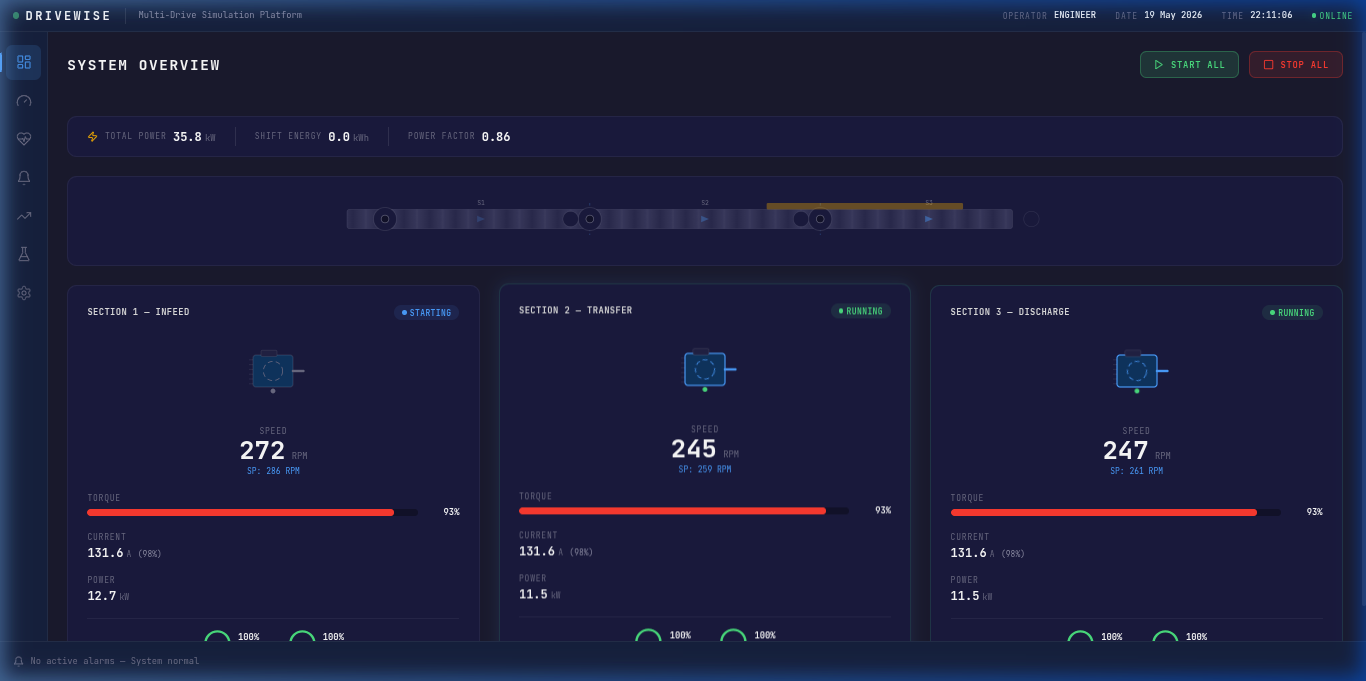
\includegraphics[width=\textwidth]{figures/overview_running.png}
        \caption{System Overview — 3 drive cards with live speed readout, torque bars, animated conveyor belt mimic with material flow, and real-time energy panel (total power, shift energy, power factor).}
        \label{fig:overview}
    \end{minipage}\hfill
    \begin{minipage}[t]{0.48\textwidth}
        \centering
        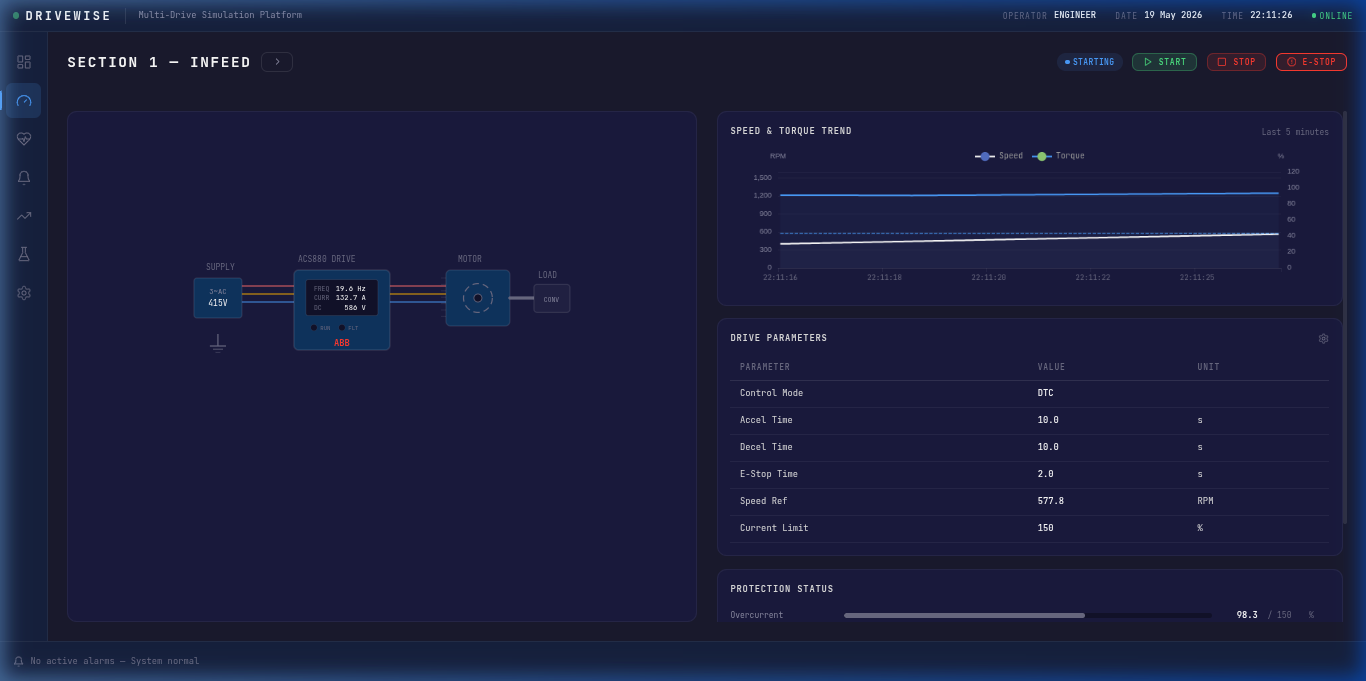
\includegraphics[width=\textwidth]{figures/detail_running.png}
        \caption{Drive Detail — Animated single-line diagram mimic showing supply, drive cabinet, motor, and load. ECharts speed/torque trend, parameter table with inline editing, protection status bars.}
        \label{fig:detail}
    \end{minipage}
\end{figure*}

\begin{figure*}[t]
    \centering
    \begin{minipage}[t]{0.48\textwidth}
        \centering
        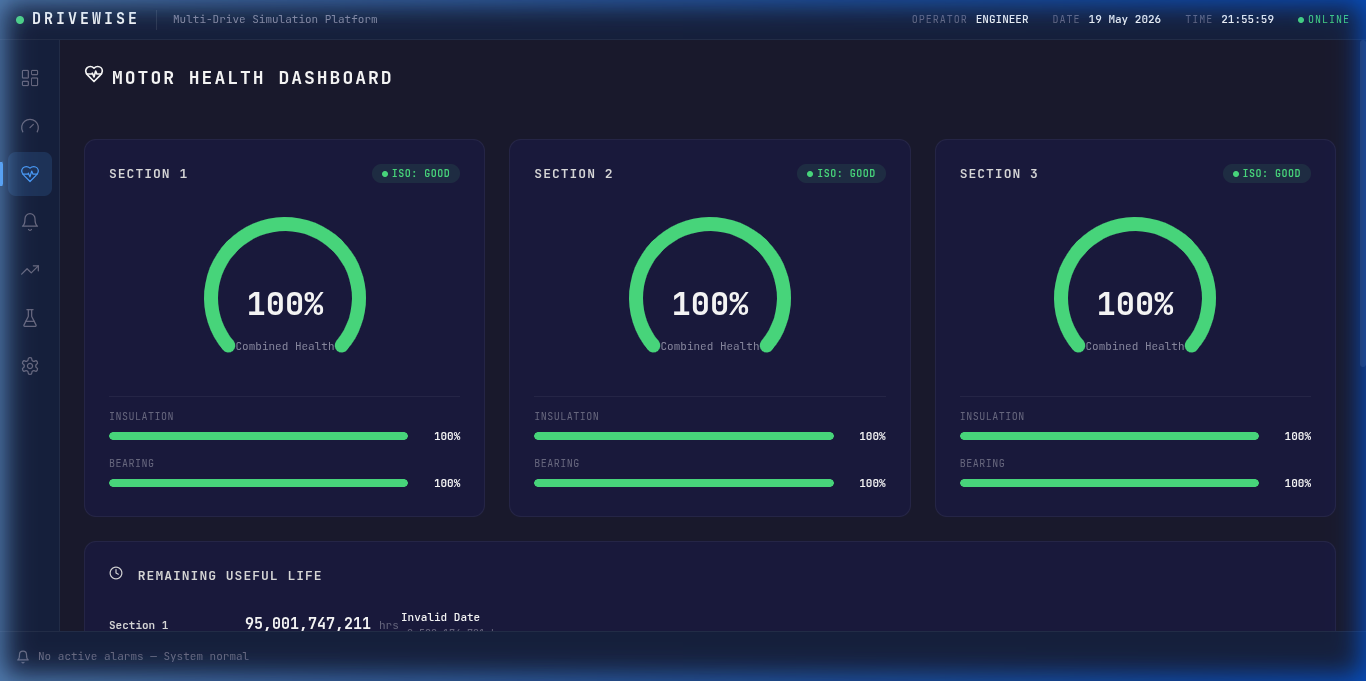
\includegraphics[width=\textwidth]{figures/health_screen.png}
        \caption{Motor Health Dashboard — Radial health gauges per motor section (combined score), insulation and bearing health bars, RUL prediction in operating hours, ISO~10816 vibration classification.}
        \label{fig:health}
    \end{minipage}\hfill
    \begin{minipage}[t]{0.48\textwidth}
        \centering
        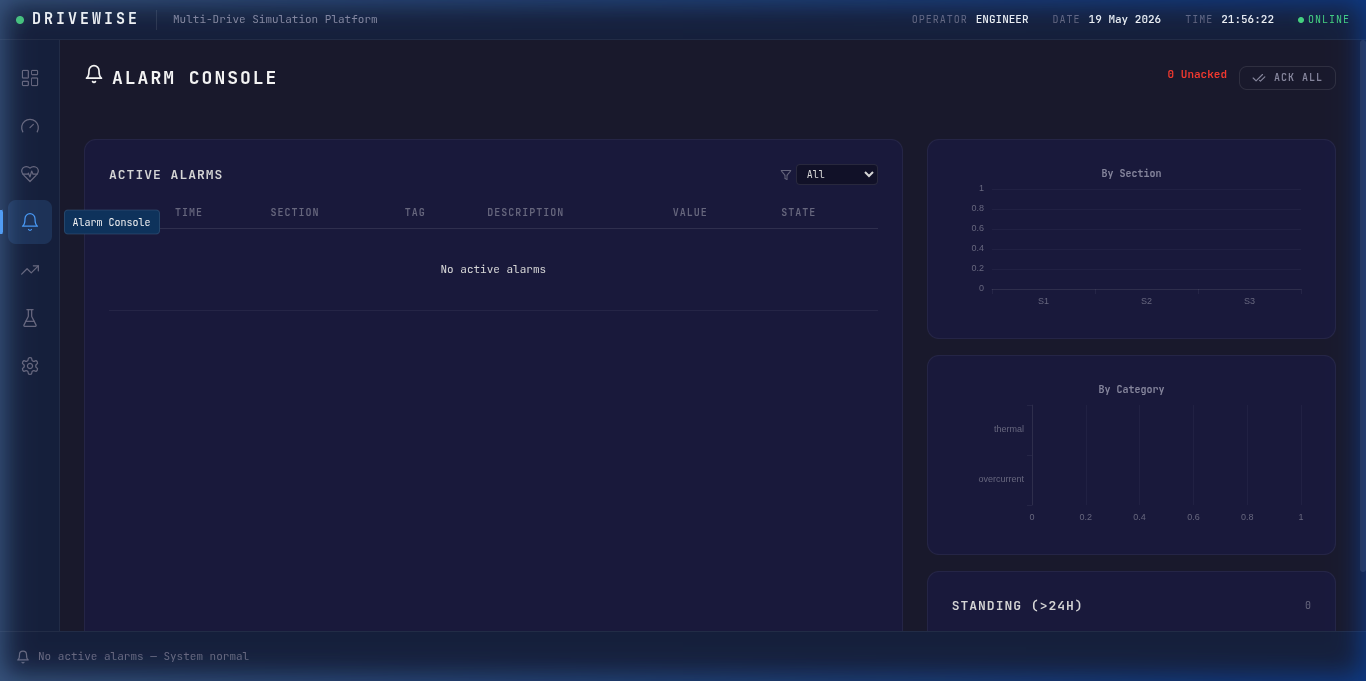
\includegraphics[width=\textwidth]{figures/alarm_screen.png}
        \caption{Alarm Console — ISA-18.2 compliant alarm list with priority filtering, alarm distribution by section and category analysis charts, acknowledge/shelve controls.}
        \label{fig:alarms}
    \end{minipage}
\end{figure*}

\begin{figure*}[t]
    \centering
    \begin{minipage}[t]{0.48\textwidth}
        \centering
        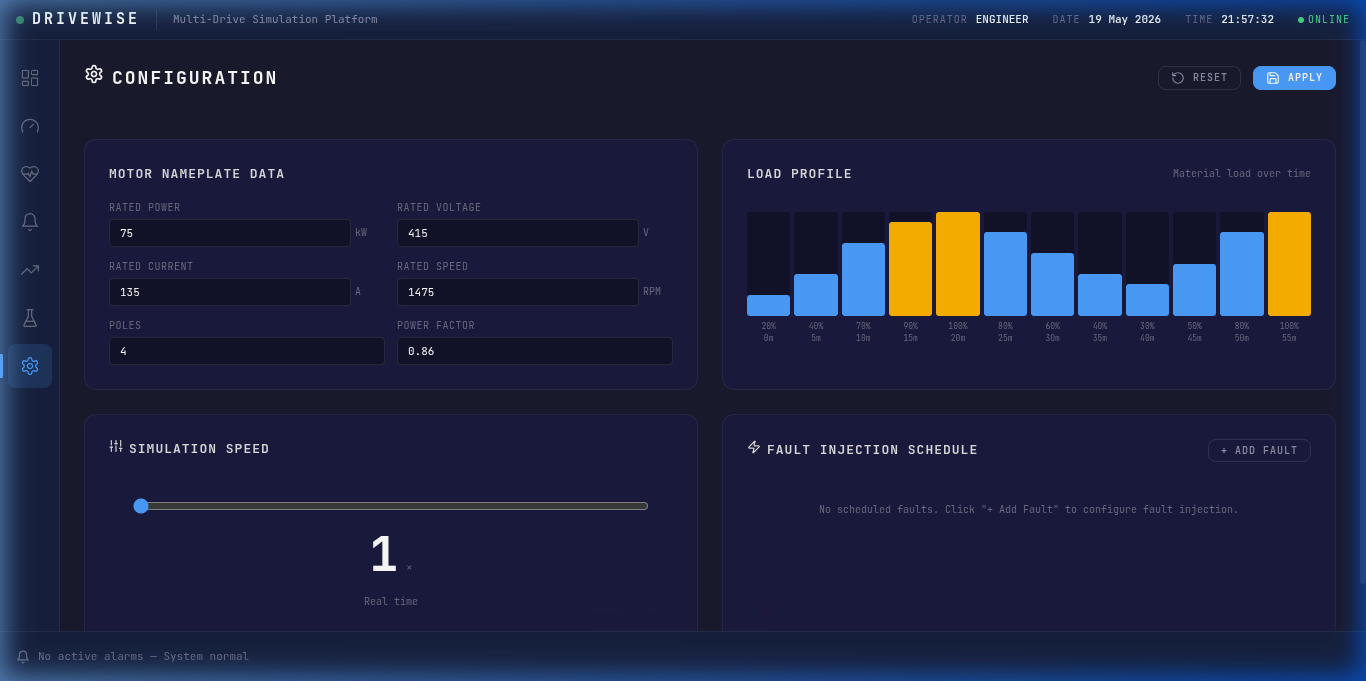
\includegraphics[width=\textwidth]{figures/config_screen.png}
        \caption{Configuration — Motor nameplate editor, live-apply load profile bars (each bar sends WebSocket update on change), simulation speed slider, fault injection schedule builder.}
        \label{fig:config}
    \end{minipage}\hfill
    \begin{minipage}[t]{0.48\textwidth}
        \centering
        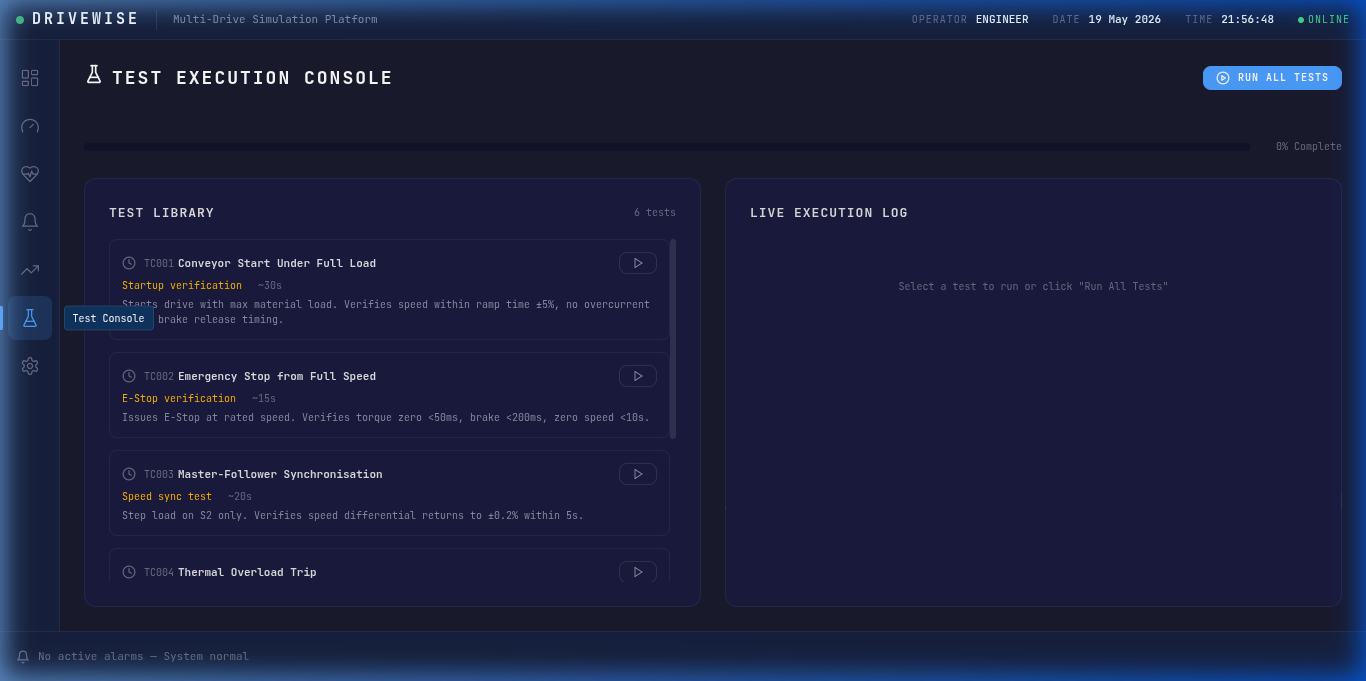
\includegraphics[width=\textwidth]{figures/test_screen.png}
        \caption{Test Execution Console — 6 FAT test cases with live execution log, per-test progress tracking, overall completion bar, and PDF report generation button.}
        \label{fig:test}
    \end{minipage}
\end{figure*}

\begin{figure*}[t]
    \centering
    \begin{minipage}[t]{0.48\textwidth}
        \centering
        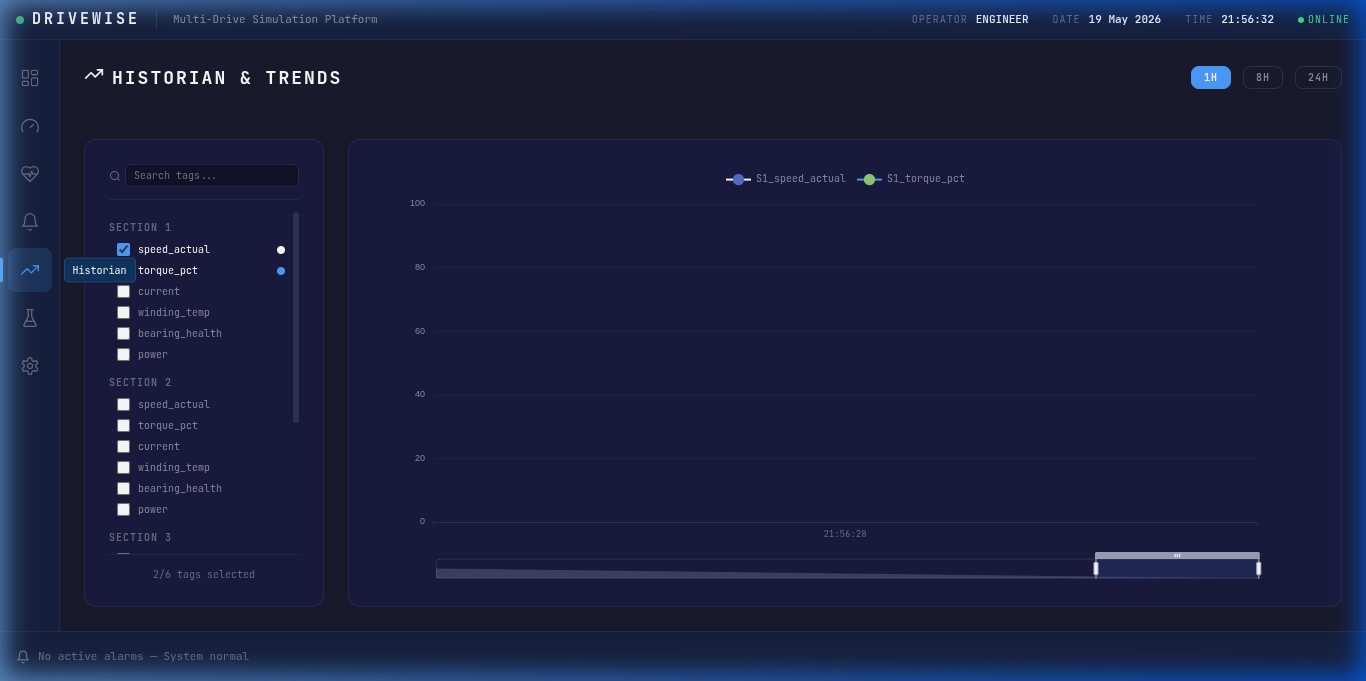
\includegraphics[width=\textwidth]{figures/historian_screen.png}
        \caption{Historian \& Trends — Multi-tag selector with real-time ECharts trend chart, time-range zoom capability, and live WebSocket data streaming at 10\,Hz update rate.}
        \label{fig:historian2}
    \end{minipage}\hfill
    \begin{minipage}[t]{0.48\textwidth}
        \centering
        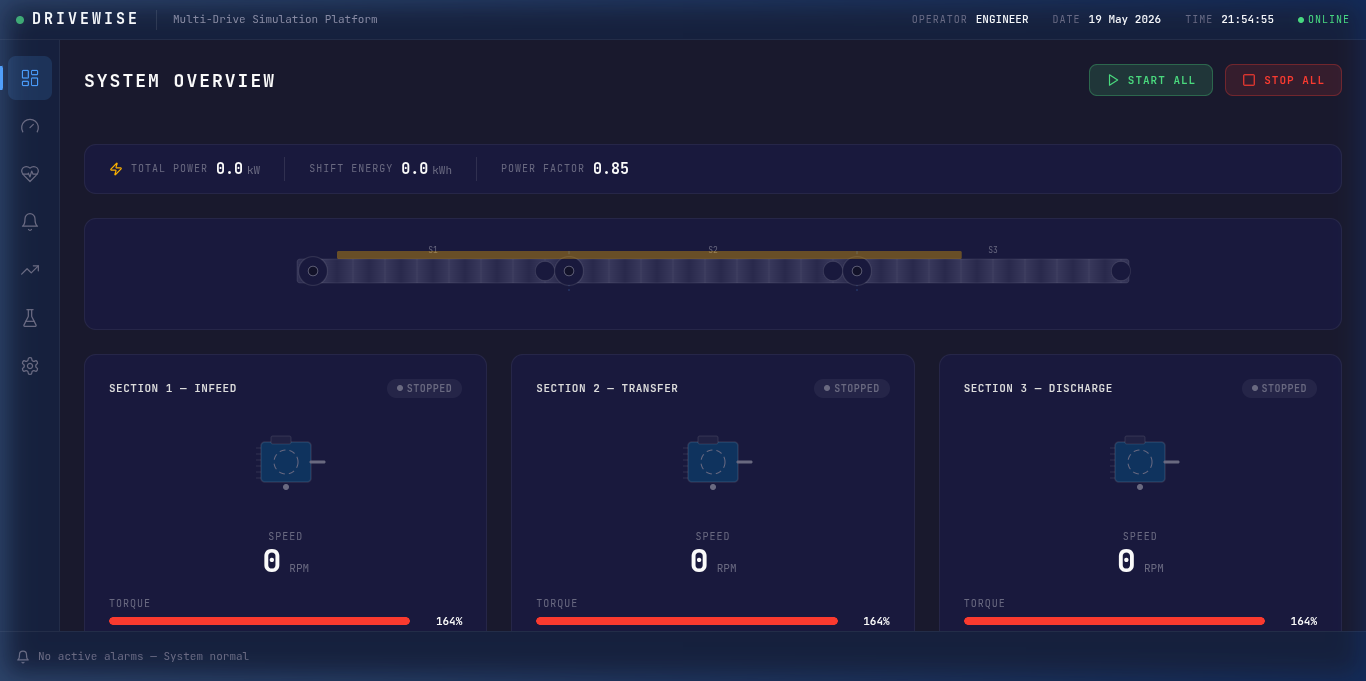
\includegraphics[width=\textwidth]{figures/overview_stopped.png}
        \caption{System Idle State — ISA-101 grey-state design in action. All drive cards show STOPPED status with zero speed and torque. Colour is completely absent, demonstrating the ``colour = abnormality'' principle.}
        \label{fig:idle}
    \end{minipage}
\end{figure*}

\subsection{Master-Follower Coordination Logic}

The simulation coordinator implements ABB's standard multi-drive coordination pattern. Section~1 (Infeed) operates as the master drive, running at the operator-set speed reference. Sections~2 and~3 receive their speed references as a configurable ratio of the master speed, with a trim adjustment to maintain belt tension.

The coordinator continuously monitors speed differentials between adjacent sections. If Section~2 runs faster than Section~1, material piles up at the transfer point. If slower, material backs up and jams. The follower control loop adjusts trim in real time to maintain the target differential — typically 0\% (matched speed) or a slight $+$0.5\% per section to keep belts taut.

When the master drive (S1) faults, the coordinator executes a fault cascade: all follower drives receive an immediate emergency stop command. This prevents the dangerous condition of downstream sections continuing to run while upstream material supply has stopped. The automated test TC006 specifically validates this cascade logic.

\subsection{Automated Factory Acceptance Testing}

The FAT test engine is the platform's most industrially significant feature. It executes 6 test cases autonomously — each test resets the simulator to a clean state, applies specific test conditions, runs the physics for the required duration, evaluates assertions against IEC-referenced pass criteria, and generates a detailed execution log with timestamps. No human intervention is required.

\begin{table}[H]
    \caption{Factory Acceptance Test Suite — 6 Automated Tests}
    \label{tab:fat}
    \begin{tabular}{@{}p{0.08\columnwidth} p{0.36\columnwidth} p{0.42\columnwidth}@{}}
    \toprule
    \textbf{ID} & \textbf{Test Name} & \textbf{Pass Criteria} \\
    \midrule
    TC001 & Start Under Full Load & Speed $\pm$5\% in ramp time, no OC trip, brake released \\
    TC002 & E-Stop from Full Speed & Torque zero $<$50\,ms, speed zero $<$10\,s \\
    TC003 & Master-Follower Sync & Speed differential $<$2\% within 5\,s of disturbance \\
    TC004 & Thermal Overload Trip & Temperature rise detected, thermal tracking active \\
    TC005 & Power Dip Ride-Through & 80\% dip: ride-through; 65\% dip: correct trip \\
    TC006 & Fault Cascade Response & S1 fault $\rightarrow$ S2, S3 stop within 500\,ms \\
    \bottomrule
    \end{tabular}
    \tabletext{Tests reference IEC~60255, IEC~61131-3, IEC~60204, IEC~61000, and ISA-18.2 standards.}
\end{table}

Upon completion, a \textbf{PDF FAT Report} is auto-generated via Python ReportLab — containing a formal cover page, executive summary table with pass/fail counts, per-test assertion tables showing expected vs.\ actual values, timestamped execution logs, and a sign-off page with Engineer/Manager/Customer fields. This matches the documentation format used in real ABB drive commissioning.

\subsection{Evaluation Criteria Mapping}

\begin{table}[H]
    \caption{Mapping to Evaluation Criteria}
    \label{tab:criteria}
    \begin{tabular}{@{}p{0.20\columnwidth} p{0.72\columnwidth}@{}}
    \toprule
    \textbf{Criterion} & \textbf{DRIVEWISE Implementation} \\
    \midrule
    \textbf{Innovation} & DTC algorithm simulation (ABB's patented technology), predictive maintenance with RUL calculation (mirrors ABB Ability Smart Sensor), automated first-out alarm detection, virtual FAT environment — none appear in standard student projects \\
    \textbf{Technical} & Dual-node thermal model, Arrhenius insulation life, IEC~60255 inverse-time curves, S-curve ramp generator, ISO~10816 bearing classification, master-follower coordination with fault cascade \\
    \textbf{Industrial} & ACS880 DTC is deployed in every ABB drive; multi-drive conveyors are ABB's largest drive market segment globally; every platform element maps directly to ABB products and workflows \\
    \textbf{Scalability} & Drive-agnostic physics layer — swap motor nameplate and load profile to simulate pump stations, crane hoists, paper machines, or wind turbine pitch drives; test suite runs identically regardless \\
    \bottomrule
    \end{tabular}
\end{table}

%===========================================================
% PAGE 5 — EXPECTED OUTPUT
%===========================================================

\section{Expected Output}

DRIVEWISE produces five concrete, demonstrable outputs — all functional and verified as a live application, not a static mockup.

\begin{note}
The platform runs as two processes: a Python simulation engine (port 8765) and a React development server (port 5173). All outputs below are operational and can be demonstrated live.
\end{note}

\paragraph{Output 1 — Real-Time Multi-Drive Simulation.}
A fully operational simulation of 3 coordinated ABB ACS880 drives controlling a bulk material conveyor system. All four physics models — drive torque control, motor thermal dynamics, conveyor inertia and friction, bearing vibration — run simultaneously at 10\,Hz update rate. Operators can start and stop drives individually or collectively, adjust parameters in real time, inject faults, and observe realistic physical responses including S-curve ramp profiles, load-dependent torque transients, and progressive thermal rise.

\paragraph{Output 2 — ISA-101 High-Performance HMI (7 Screens).}
A complete SCADA-grade operator interface consisting of: (1)~System Overview with animated conveyor belt and 3 live drive cards, (2)~Drive Detail with animated single-line diagram mimic and ECharts trending, (3)~Motor Health dashboard with radial gauges showing insulation, bearing, and combined health with RUL predictions, (4)~ISA-18.2 Alarm Console with priority filtering and distribution analysis, (5)~Historian with multi-tag trend selection and time-range zoom, (6)~Test Execution Console with live logging, and (7)~Configuration panel with live-apply controls for simulation speed, load profile, motor nameplate, and fault injection.

\paragraph{Output 3 — Automated FAT Test Suite (6 Tests).}
Six Factory Acceptance Tests execute without human intervention: conveyor start under full load, emergency stop from rated speed, master-follower speed synchronisation, thermal overload trip verification, power dip ride-through vs.\ trip discrimination, and fault cascade response. Each test autonomously resets the simulator, applies test conditions, runs the physics engine, evaluates assertions against IEC-referenced criteria, and generates detailed execution logs with timestamped pass/fail results.

\paragraph{Output 4 — PDF FAT Report.}
An automatically generated A4 PDF document conforming to industrial FAT documentation standards — featuring a formal cover page with project metadata, executive summary table with overall pass/fail verdict, per-test assertion tables comparing expected and actual values, timestamped execution logs, and a sign-off page with designated fields for Test Engineer, Project Manager, and Customer Representative. This format directly matches ABB's commissioning documentation workflow.

\paragraph{Output 5 — Predictive Maintenance Analytics.}
Three health indicators per motor that decline realistically over simulated operating time: insulation health calculated from Arrhenius thermal degradation, bearing health derived from vibration spectrum analysis with ISO~10816 severity classification, and a combined Remaining Useful Life expressed in operating hours. This directly mirrors the core functionality of ABB's commercial product — the ABB Ability Smart Sensor — which performs identical analytics on real motors.

\subsection{Demonstration Capability}

The platform is fully operational and can be demonstrated live in two terminal commands:

\begin{enumerate}
    \item Start the Python simulation engine: \texttt{python3 backend/main.py}
    \item Start the React HMI: \texttt{npm run dev}
\end{enumerate}

All five outputs listed above are immediately observable. The operator can start drives, watch S-curve ramp profiles, trigger faults, observe cascade responses, run automated tests, and generate a PDF report — all in a single integrated session. The entire platform runs locally with no external dependencies or cloud connectivity required.

\begin{tauenv}[frametitle=Why DRIVEWISE Matters — The Industrial Perspective]
DRIVEWISE is not a motor animation with a speed slider. It is a \textbf{virtual commissioning environment} — the concept that ABB, Siemens, and Schneider Electric are investing billions to develop. A drive system validated in DRIVEWISE before hardware procurement means: \textbf{zero commissioning surprises} (protection curves, ramp profiles, and coordination logic verified in software), \textbf{reduced site time} (FAT tests run in minutes instead of days, with traceable PDF documentation), \textbf{predictive maintenance training} (operators learn to interpret health dashboards and RUL predictions before real equipment arrives on site), and \textbf{application portability} (the same physics engine simulates any motor-driven load — pumps, cranes, paper machines, wind turbines — by changing nameplate parameters and load profiles).
\end{tauenv}

\end{document}
